\documentclass[11pt]{article}

\usepackage[english]{babel}
\usepackage[margin=0.8in]{geometry}

% Math/Greek packages
\usepackage{amssymb,amsmath,amsthm, mathtools} 
\usepackage{algorithm, algorithmic}
\usepackage{upgreek, siunitx}
\usepackage{setspace}

% Graphics/Presentation packages
\usepackage{multirow}
\usepackage{graphicx}
\usepackage{cancel}
\usepackage{tabulary, enumitem, array}
\usepackage{xparse,mleftright,tikz}
\usepackage{physics}

% Misc packages
\usepackage{fancyhdr}


\usepackage[export]{adjustbox}

\usepackage{esint}

\sisetup{locale=US,group-separator = {,}}
\usepackage[colorlinks=true, allcolors=blue]{hyperref}


% Box function - update this as more sophisticated solutions are found
\newcommand\mybox[2][]{\tikz[overlay]\node[fill=blue!20,inner sep=2pt, anchor=text, rectangle, rounded corners=1mm,#1] {#2};\phantom{#2}}
\renewcommand{\arraystretch}{1.2}

% General macro declarations


\makeatletter
\let\oldabs\abs
\def\abs{\@ifstar{\oldabs}{\oldabs*}}
%
\let\oldnorm\norm
\def\norm{\@ifstar{\oldnorm}{\oldnorm*}}
\makeatother

\begin{document}

\title{PHSX 491: HW03}
\author{William Jardee}
\maketitle

\section*{Question 1}
\begin{enumerate}[label=\alph*)]
\item
We know that we will need to take all nine combinations of coordinates and derivatives, so let's just calculate them all out right away:

\begin{align*}
\pdv{x}{r} & = \sin(\theta)\cos(\phi) & \pdv{y}{r} & = \sin(\theta)\sin(\phi) & \pdv{z}{r} & = \cos(\theta)&\\
\pdv{x}{\theta} & = r \cos(\theta)\cos(\phi) & \pdv{y}{\theta} & = r\cos(\theta)\sin(\phi) & \pdv{z}{\theta} & = -r\sin(\theta)&\\
\pdv{x}{\phi} &= -r\sin(\theta)\sin(\phi) & \pdv{y}{\phi} &= r \sin(\theta)\cos(\phi) & \pdv{z}{\phi} &= 0&\\
\end{align*}

Now, we can use the definition of a tensor to calculate the elements one by one. Since it is just a lot of computation, I will just rapid-fire them. 
\begin{align*}
g_{\alpha^\prime \beta^\prime} = \pdv{\alpha}{\alpha^\prime}\pdv{\beta}{\beta^\prime}g_{\alpha\beta}
\end{align*}

\begin{flalign*}
g_{rr} & = \pdv{x}{r}\pdv{x}{r}g_{xx} + \pdv{x}{r}\pdv{y}{r}g_{xy} + \pdv{x}{r}\pdv{z}{r}g_{xz} + \pdv{y}{r}\pdv{x}{r}g_{yx} + \pdv{y}{r}\pdv{y}{r}g_{yy} + \pdv{y}{r}\pdv{z}{r}g_{yz} + \pdv{z}{r}\pdv{x}{r}g_{zx} &\\
& \qquad +\pdv{z}{r}\pdv{y}{r}g_{zy} + \pdv{z}{r}\pdv{z}{r}g_{zz} \\ 
& = \left[ \pdv{x}{r}\right]^2 g_{xx} +  \left[ \pdv{y}{r}\right]^2 g_{yy} +  \left[ \pdv{z}{r}\right]^2 g_{zz}\\
& = \sin[2](\theta) \cos[2](\phi) + \sin[2](\theta) \sin[2](\phi) + \cos[2](\theta)\\
& = \sin[2](\theta) + \cos[2](\theta) = 1\\
\end{flalign*}
\begin{flalign*}
g_{r\theta} & = \pdv{x}{r}\pdv{x}{\theta} g_{xx} + \pdv{y}{r}\pdv{y}{\theta}g_{yy} + \pdv{z}{r}\pdv{z}{\theta}g_{zz} = g_{\theta r}&\\
& = [\sin(\theta)\cos(\phi)][r\cos(\theta)\cos(\phi)] + [\sin(\theta)\sin(\phi)][r\cos(\theta)\sin(\phi)] + [\cos(\theta)][-r\sin(\theta)]\\
& = r\sin(\theta)\cos(\theta)\cos[2](\phi) + r \sin(\theta)\cos(\theta)\sin[2](\phi) -r\cos(\theta)\sin(\theta)\\
& = r\sin(\theta)\cos(\theta) - r \cos(\theta)\sin(\theta) = 0
\end{flalign*}
\begin{flalign*}
g_{r\phi} & = \pdv{x}{r}\pdv{x}{\phi}g_{xx} + \pdv{y}{r}\pdv{y}{\phi}g_{yy} + \pdv{z}{r}\pdv{z}{\phi}g_{zz} = g_{\phi r} &\\
& = [\sin(\theta)\cos(\phi)][-r\sin(\theta)\sin(\phi)] + [\sin(\theta)\sin(\phi)][r\sin(\theta)\cos(\phi)] + 0 =0
\end{flalign*}
\begin{flalign*}
g_{\theta\phi} & = \pdv{x}{\theta}\pdv{x}{\phi}g_{xx} + \pdv{y}{\theta}\pdv{y}{\phi}g_{yy} + \pdv{z}{\theta}\pdv{z}{\phi}g_{zz} = g_{\phi \theta} &\\
& = [r\cos(\theta)\cos(\phi)][-r\sin(\theta)\sin(\phi)] + [r\cos(\theta)\sin(\phi)][r\sin(\theta)\cos(\phi)] + 0 = 0
\end{flalign*}
\begin{flalign*}
g_{\theta\theta} & = \left[ \pdv{x}{\theta}\right]^2 g_{xx} +  \left[ \pdv{y}{\theta}\right]^2 g_{yy} +  \left[ \pdv{z}{\theta}\right]^2 g_{zz} &\\
& = [r\cos(\theta)\cos(\phi)]^2 +[r \cos(\theta)\sin(\phi)]^2 + [-r\sin(\theta)]^2\\
& = r^2 \cos[2](\theta)\cos[2](\phi) + r^2 \cos[2](\theta)\sin[2](\phi) + r^2\sin[2](\theta)\\
& = r^2\cos[2](\theta) + r^2\sin[2](\theta) = r^2
\end{flalign*}
\begin{flalign*}
g_{\phi\phi} & = \left[ \pdv{x}{\phi}\right]^2 g_{xx} +  \left[ \pdv{y}{\phi}\right]^2 g_{yy} +  \left[ \pdv{z}{\phi}\right]^2 g_{zz} &\\
& = [-r\sin(\theta)\sin(\phi)]^2 + [r\sin(\theta)\cos(\phi)]^2 + [0]^2\\
& = r^2\sin[2](\theta)\sin[2](\phi) + r^2\sin[2](\theta)\cos[2](\phi) = r^2\sin[2](\theta)\\
\end{flalign*}

\[\boxed{g_{\alpha^\prime \beta^\prime} = \mqty[1 & 0 & 0 \\ 0 & r^2 & 0 \\ 0 & 0 & r^2\sin[2](\theta)]}\]
Where the coordinates $\alpha^\prime, \beta^\prime$ are in $(r, \theta, \phi)$. 

\item We know that the inverse of a diagonal matrix is that matrix with each diagonal element replaced with its reciprocal:
\[\boxed{g^{\alpha^\prime \beta^\prime} = \mqty[1 & 0 & 0 \\ 0 & \frac{1}{r^2} & 0 \\ 0 & 0 & \frac{1}{r^2\sin[2](\theta)}]}\]

\item Let's be nit-picky and calculate the covector of the vector. This should be the transpose of the vector, and indeed it is.
$A_x = 1 \cdot g_{xx} + 1 \cdot g_{xy} + 1 \cdot g_{xz} = 1$\\
$A_y = 1 \cdot g_{yx} + 1 \cdot g_{yy} + 1 \cdot g_{yz} = 1$\\
$A_z = 1 \cdot g_{zx} + 1 \cdot g_{zy} + 1 \cdot g_{zz} = 1$

\[\boxed{\tilde{A} = \mqty[1 & 1 & 1]}\]

Invoking the dot-product:\\
$A^2 = A^\alpha g_{\alpha \beta}A^\beta = A^\alpha A_\alpha = 3$
\[\boxed{A^2 = 3}\]

\item In order to find the magnitude in spherical coordinates, we must transform the vector into those coordinates. Here is the general equation for transforming Cartesian to spherical coordinates:
\begin{align*}
r &= \sqrt{x^2 + y^2 + z^2} & \theta & = \tan[-1](\frac{y}{x}) & \phi & = \tan[-1](\frac{\sqrt{x^2 + y^2}}{z})
\end{align*}

Doing this calculation:
\[\vec{A} \longrightarrow \mqty[\sqrt{3} \\ \frac{\pi}{4} \\ \tan[-1](\sqrt{2})]\]

Calculating the covector in spherical:
\[A_\alpha = g_{\alpha \beta} A^{\beta}\]
\begin{flalign*}
A_r & = \sqrt{3} \cdot g_{rr} + \frac{\pi}{4}\cdot g_{r \theta} + \tan[-1](\sqrt{2})g_{r\phi} = \sqrt{3}&\\
A_\theta & = \sqrt{3} \cdot g_{\theta r} + \frac{\pi}{4}g_{\theta \theta} + \tan[-1](\sqrt{2})g_{\theta\phi} = r^2\frac{\pi}{4}\\
A_\phi & = \sqrt{3} \cdot g_{\phi r} + \frac{\pi}{4}g_{\phi \theta} + \tan[-1](\sqrt{2})g_{\phi\phi} = r^2\sin[2](\theta)\tan[-1](\sqrt{2})
\end{flalign*}
\[\boxed{\tilde{A} = \mqty[\sqrt{3} & r^2\frac{\pi}{4} & r^2\sin[2](\theta)\tan[-1](\sqrt{2})]}\]

Calculating the magnitude in the spherical:
\begin{flalign*}
A_\alpha A^\alpha & = A_r A^r + A_\theta A^\theta + A_\phi A^\phi & \\
& = \sqrt{3}\cdot \sqrt{3} + \frac{\pi}{4}\cdot r^2 \cdot\frac{\pi}{4} + \tan[-1](\sqrt{2})\cdot r^2\sin[2](\theta)\cdot \tan[-1](\sqrt{2})
\end{flalign*}

To measure the magnitude we will need to orientate the vector at the origin. At the origin $r = 0$, and thus the latter two terms drop out. So, the magnitude is:
\[\boxed{A^2 = 3}\]

\item From this one example this is pretty strong extrapolation, but logically it makes sense that when we transform coordinates the length is \underline{invariant}.


\end{enumerate}

\section*{Question 2}
\begin{figure}[!ht]
\centering
	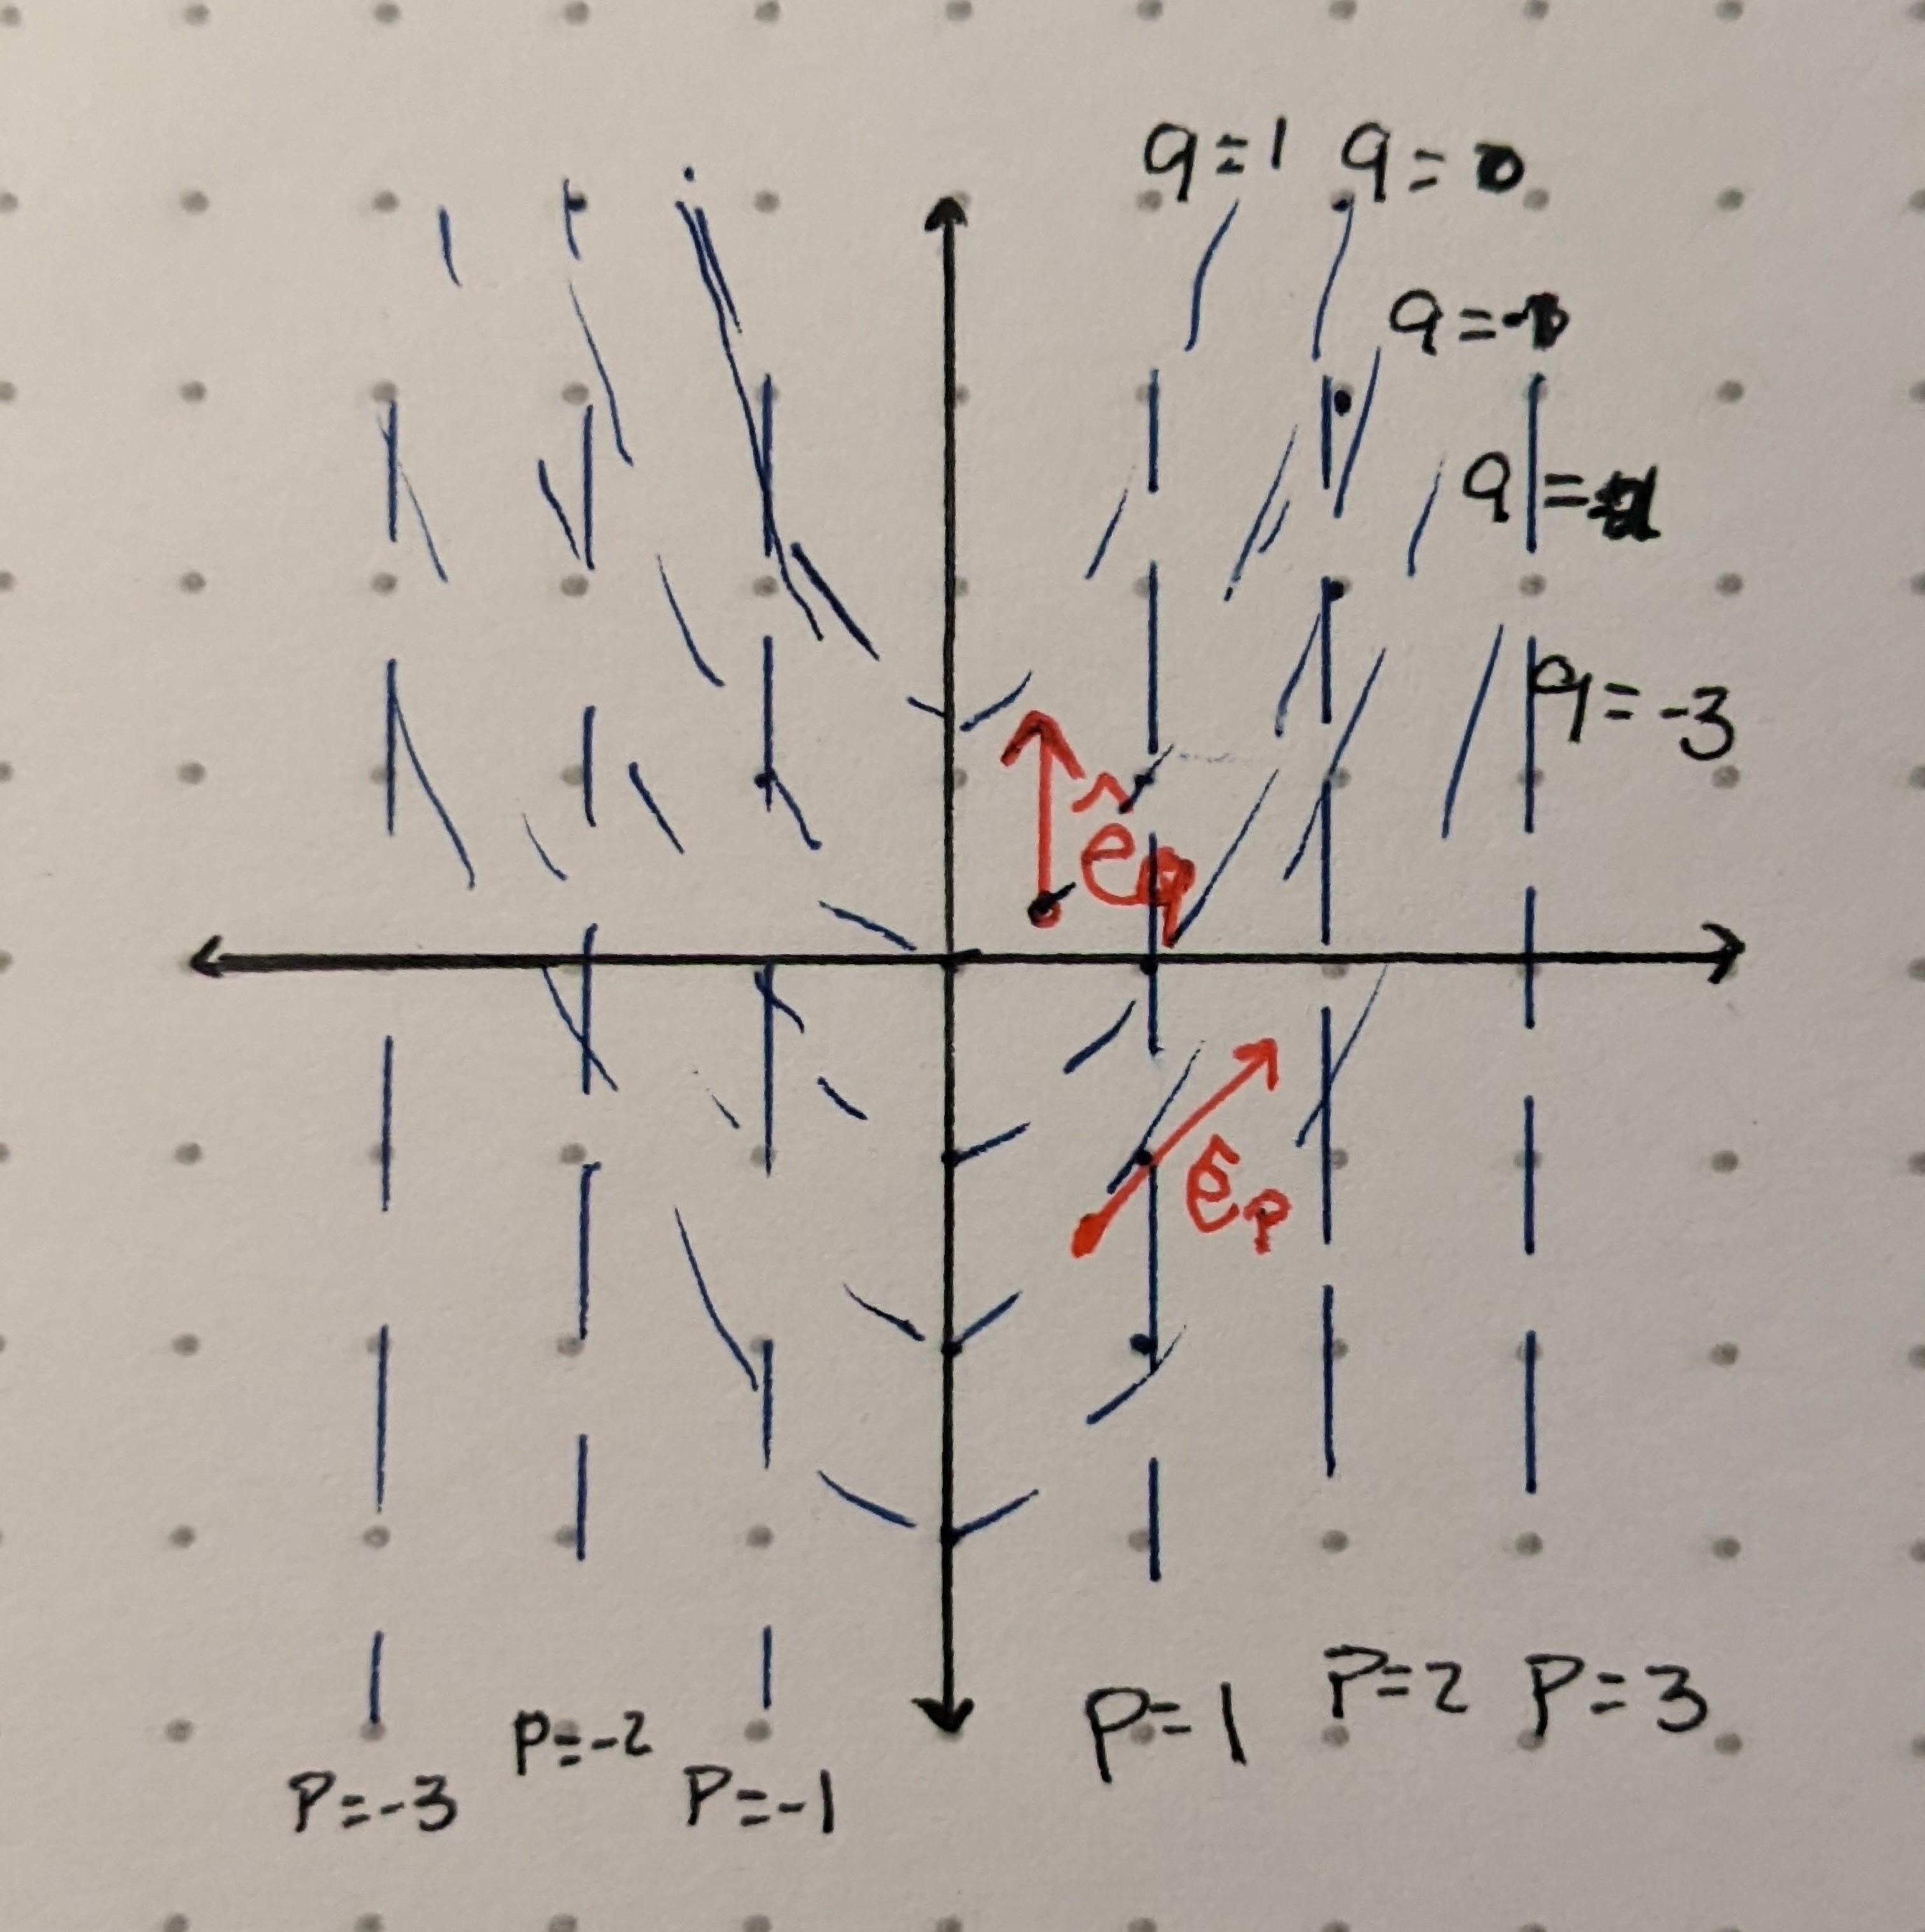
\includegraphics[width=0.5\textwidth]{phsx491_hw04_01.jpg}
	\caption{Our new $p-q$ coordinates. Constant $q$ looks like a parabola, and constant $p$ are values of $x$.}
	\label{fig:2.1}
\end{figure}

\begin{enumerate}[label=\alph*)]
\item See Fig.~\ref{fig:2.1}
\item 
\begin{align*}
q &= y -cx^2 = y-cp^2 \\
\rightarrow y &= q+ cp^2
\end{align*}
\[\boxed{\mqty{x(p,q) = p \\ y(p,q) = q + cp^2}}\]
\item 
If we ``zoom" into a point, the smoothness of the space allows us to use the Pythagorean theorem:
\begin{align*}
\dd{s^2} & \approx \dd{x^2} + \dd{y^2}\\
&= \left(\dd{p}\right)^2 + \left(\dd{q} + 2cp \dd{p}\right)^2\\
&= \left(\dd{p}\right)^2 + \left(\dd{q}\right)^2 + 4cp\dd{p}\dd{q} + 4c^2 p^2 \left(\dd{p}\right)^2
\end{align*}
Using this to find the tensor definition of the dot product and assuming that $g_{pq} = g_{qp}$:
\begin{align*}
g_{\alpha \beta} \dd{x}^\alpha \dd{x}^\beta & \rightarrow g_{pp}\left(\dd{p}\right)^2 + g_{pq}\dd{p}\dd{q} + g_{qp} \dd{q} \dd{p} + g_{qq} \left(\dd{q}\right)^2\\
\left(1 + 4c^2p^2\right)\left(\dd{p}\right)^2 + 4cp\dd{p}\dd{q} + \left(\dd{q}\right)^2 & = g_{pp}\left(\dd{p}\right)^2 + 2g_{pq}\dd{p}\dd{q} + g_{qq} \left(\dd{q}\right)^2\\
g_{pp} & = 1 + 4c^2p^2\\
g_{pq} & = 2cp\\
g_{qq} & = 1 \\
\end{align*}
 
Putting this into a matrix representation of the tensor:
\[\boxed{M_{qp} = \mqty[1 & 2cp \\ 2cp & 1+4c^2p^2]}\]

\item
The primary takeaways is that {\bf a)} the vectors are not \underline{orthogonal} (this is from the fact that off diagonal elements are not zero) and {\bf b)} that $\hat{e}_p$ is not normalized (a.k.a. the basis is not ortho\underline{normal}).

\end{enumerate}

\end{document}
